\documentclass{article}
\author{RustColeone}
\usepackage{amsmath}
\usepackage{amssymb}
\usepackage{amsfonts}
\usepackage{enumitem}
\usepackage{titling}
\usepackage{aligned-overset}
\usepackage{tikz}
\usepackage{wrapfig}
\usepackage{hyperref}
\usepackage{pgffor}
\usepackage{pgfplots}
\usepackage{verbatim}
\usepackage{tabularx}
%\setlength{\droptitle}{-12em}
\title{Math, Multivariable Calculus}
\setlength{\parindent}{0pt}
\newlength\tindent
\setlength{\tindent}{\parindent}
\setlength{\parindent}{0pt}
\renewcommand{\indent}{\hspace*{\tindent}}
\newcommand{\tab}[1]{
    \foreach \n in {1,...,#1}{\;\;\;\;}
}
\newcommand{\n}{$\\$}
\newcommand{\VectorTwo}[2]{
    \left[
        \begin{array}{c}
            #1\\
            #2
        \end{array}
    \right]
}
\newcommand{\R}{\rm I\!R}
\newcommand{\parallelsum}{\mathbin{\!/\mkern-5mu/\!}}


\begin{document}
\maketitle
\newpage
\tableofcontents
\newpage
\section{Vectors}
    \subsection{Vector Calculations}
\section{Vector functions}
    \subsection{Vector Valued functions in multiple variables}
        Calculus of single variable is a study of $y=f(x)$
        \begin{align}
            y=f(x)\text{, where\;} (x\in\R)\rightarrow(f(x)\in\R)\\
        \end{align}
        However, when we are dealing with multi-variable calculus, we have: an n variable vector valued function (if $m > 1$)
        \begin{equation}
            F=
            \begin{cases}
                (x_1,\dots x_n)&\rightarrow F(x_1,\dots x_n)\\
                \text{\tab{1}}\in&\text{\tab{3}\;}\in\\
                \text{\tab{1}}\R^n&\longrightarrow\text{\tab{1}\;\;\;}\R^m\\
            \end{cases}
        \end{equation}
        where $F(x_1,\dots,x_n)=(F_1(x_1,\dots,x_n),\; F_2(x_1,\dots,x_n)\dots F_m(x_1,\dots,x_n))$\n
        The inputs and ouputs are Vectors, for example
        \begin{align}
            d(x,y) &= \sqrt{x^2+y^2}, (2 variables)\\
            (x,y)\R^2&\rightarrow(\sqrt{x^2+y^2})\R\\
            distance &= \sqrt{x^2+y^2}
        \end{align}
        \begin{center}
            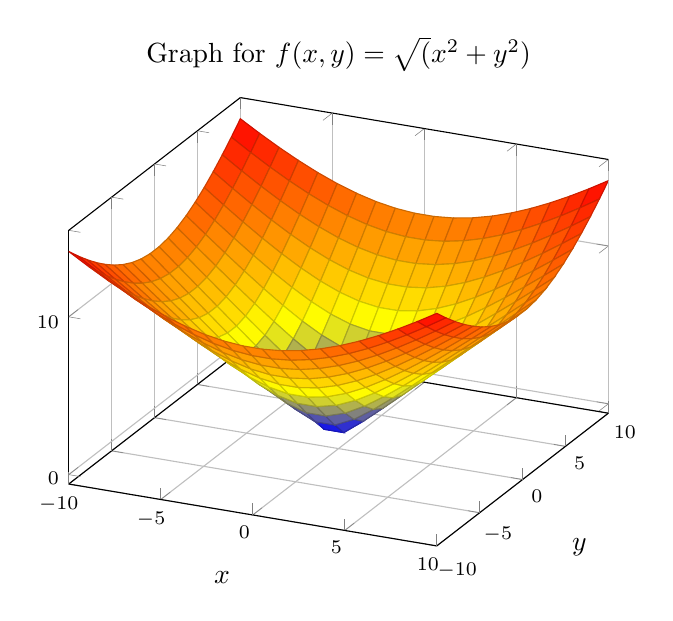
\begin{tikzpicture}
                \begin{axis} [
                    title = {Graph for $f(x,y) = \sqrt(x^2+y^2)$},
                    xtick = {-10,-5,...,10},
                    ytick = {-10,-5,...,10},
                    xlabel = $x$, ylabel = $y$,
                    ticklabel style = {font = \scriptsize},
                    grid
                ]
                \addplot3 [surf, domain=-10:10, samples=20] 
                    { sqrt(x^2 + y^2) };
                \end{axis}
            \end{tikzpicture}
        \end{center}
        \begin{center}The graph should look like a cone\end{center}
        Similarly, we can have a function that takes all the x, y and z can calculate that distance. That would however be a four dimensional plot, which we cannot plot.
        
        For a similar function, $z=x^2+y^2$\n
        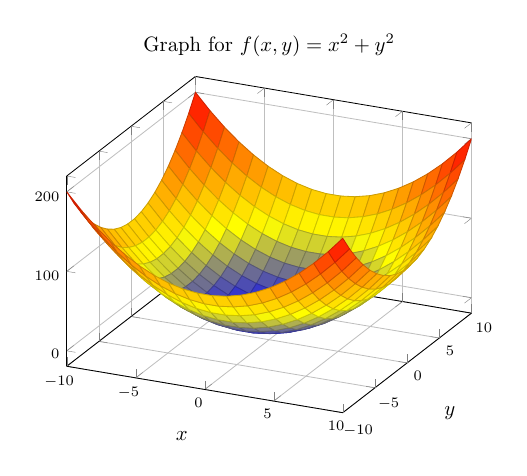
\begin{tikzpicture}[scale=0.75]
            \begin{axis} [
                title = {Graph for $f(x,y) = x^2+y^2$},
                xtick = {-10,-5,...,10},
                ytick = {-10,-5,...,10},
                xlabel = $x$, ylabel = $y$,
                ticklabel style = {font = \scriptsize},
                grid
            ]
            \addplot3 [surf, domain=-10:10, samples=20] 
                { x^2 + y^2 };
            \end{axis}
        \end{tikzpicture}
        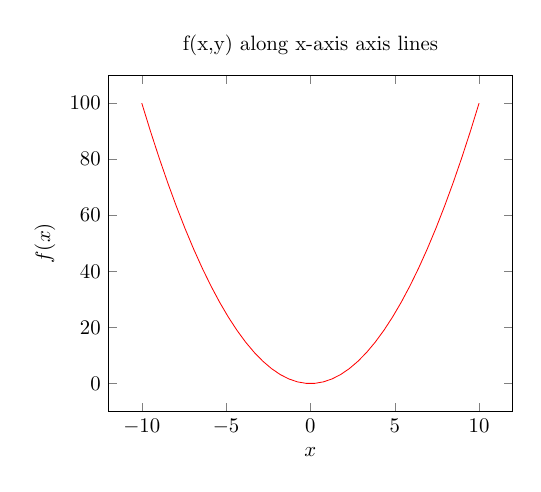
\begin{tikzpicture}[scale=0.75]
            \begin{axis}[
                title = {f(x,y) along x-axis}
                axis lines = left,
                xlabel = $x$,
                ylabel = {$f(x)$},
            ]
            \addplot [
                domain=-10:10, 
                samples=40, 
                color=red,
            ]
                {x^2};
            \end{axis}
        \end{tikzpicture}
        For another function $f(z) = (\cos{z},\sin{z})$\n
        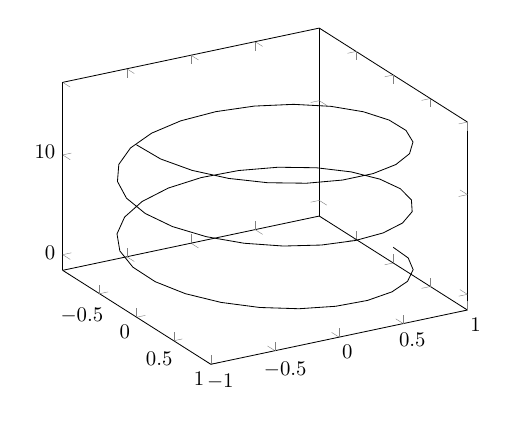
\begin{tikzpicture}[scale = 0.75]
            \begin{axis}
            [
                view={60}{30},
            ]
            \addplot3[
                domain=0:5*pi,
                samples = 60,
                samples y=0,
            ]
            ({sin(deg(x))}, {cos(deg(x))}, {x});
            \end{axis}
        \end{tikzpicture}
        \resizebox{5.5cm}{5cm}{
            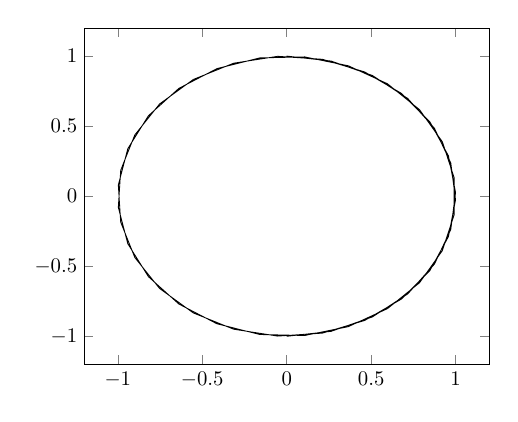
\begin{tikzpicture}[scale = 0.75]
                \begin{axis}
                [
                    view={60}{30},
                ]
                \addplot[
                    domain=0:5*pi,
                    samples = 60,
                    samples y=0,
                ]
                ({sin(deg(x))}, {cos(deg(x))});
                \end{axis}
            \end{tikzpicture}
        }
    \subsection{Limits and continuity}
        Definition:
        \begin{align}
            &\lim_{(x,y) \rightarrow (a,b)} f(x,y) = L\\
            &\text{if\;} f(x,y) \text{\;goes to L as\;}(x,y) \text{\;approaches\;}(a,b)\nonumber
        \end{align}
        \begin{center}
            \begin{tikzpicture}[scale = 0.7]
                \begin{axis}[
                    title = {continuous}
                    xlabel = $x$,
                    ylabel = {$f(x)$},
                    label = {a}
                ]
                \addplot [
                    domain=-2.5:2.5, 
                    samples=22, 
                    color=red,
                ]{-x^3};
                \end{axis}
            \end{tikzpicture}
            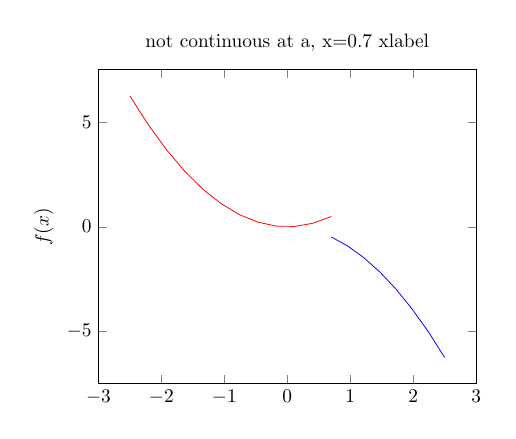
\begin{tikzpicture}[scale = 0.7]
                \begin{axis}[
                    title = {not continuous at a, x=0.7}
                    xlabel = $x$,
                    ylabel = {$f(x)$},
                ]
                \addplot [
                    domain=-2.5:0.7, 
                    samples=12, 
                    color=red,
                ]{x^2};
                \addplot [
                    domain=0.7:2.5, 
                    samples=8, 
                    color=blue,
                ]{-x^2};
                \end{axis}
            \end{tikzpicture}
            $\lim_{(x\rightarrow a^+)}f(x)=\lim_{(x\rightarrow a^-)}f(x)$, \tab{3}$\lim_{(x\rightarrow a^+)}g(x)$ DNE
        \end{center}
        Similarly, for $(x,y)\rightarrow(a,b)$ we need to look at all possible paths. If you can find 2 oaths to approach (a,b) such limits along these 2 paths are different, then the function is not continuous. For example:
        \begin{align}
            \lim_{(x,y) \rightarrow (0,0)} \frac{2xy}{x^2+y^2} &=  \text{DNE(do not exists) since:}\\
            (x,0) \rightarrow (0,0),\;\lim=\lim_{x\rightarrow0} &=\frac{0}{x^2}= 0\\
            (x,x) \rightarrow (0,0),\;\lim=\lim_{y\rightarrow0} &=\frac{2x*x}{x^2+x^2}= 1\\
            1&\neq 0\text{\;hence D.N.E.}\nonumber
        \end{align}
        Remember to take a look at all directions
        
        Definition: $f(x,y)$ continuous at $(a,b)$ if:
        \begin{enumerate}
            \item $f(x,y)$ defined at $(a,b)$
            \item $\lim_{(x,y)\rightarrow(a,b)} = f(a,b)$
        \end{enumerate}
        How to tell if a function is continuous?
        $f(x,y,z) = e^{x-z}\sin(x+yz^2)$
        \begin{enumerate}
            \item \begin{enumerate}
                    \item $f(x,y,z) = x$
                    \item $f(x,y,z) = y$
                    \item $f(x,y,z) = z all continuous$
                \end{enumerate}
            \item $f(x,y,z) = x-z$
            \item $f(x,y,z) = e^{x-z}(composition of contin.func is contin.)$
            \item $g(x,y,z) = \sin(x+yz^2)$ continuous similarly
        \end{enumerate}
        Test: $\lim_{(x,y,z)\rightarrow(0,1,-1)} = e^1\sin{(1)}$, hence continuous. A special case is when you have $\frac{f(x,y)}{g(x,y)}$, it will be continuous at (a,b) as long as $g(a,b) \neq 0$
        
        For a vector function $F(\vec{v}) = (F_1(\vec{v}),F_2(\vec{v}\dots F_m(\vec{v})$, where $\vec{v}$ is a vector or $\R^n, (x_1,x_2\dots x_n)$, is a continuous function at vector $\vec{n}$ if all its component functions are continuous at $\vec{n}$
        
        Example:
        \begin{align}
            f(x,y,z) = (e^{x+y},\;z,\;\cos(x^2-z)) \text{\;continuous everywhere}\\
            \text{since}\begin{cases}
                e^{x+y} \text{\;continuous} \\
                z \text{\;continuous} \\
                \cos(x^2-z) \text{\;continuous}
            \end{cases}
        \end{align}
    
    \subsection{Partial Derivatives}
        The derivative of a function is the rate of change along the x axis. The partial derivatives of $F(x,y)$ would be the rate of change of F as one of the axis is fixed (along one axis).
        \begin{align}
            \frac{dF(x,y)}{dx} = F_x(x,y) = \lim_{\Delta x \rightarrow 0}\frac{F(x+\Delta x,y)-F(x,y)}{\Delta x}\\
            \frac{dF(x,y)}{dy} = F_y(x,y) = \lim_{\Delta y \rightarrow 0}\frac{F(x,y+\Delta y)-F(x,y)}{\Delta y}
        \end{align}
        In order to compute the derivative, we treat all other variables as constants.
        
        Example:
        \begin{align}
            f(x,y,z) = xe^{xy}-\sin{(y^2+z^2)}\\
            \frac{df}{dx} = e^{xy}+yxe^{xy}-0=e^{xy}+yxe^{xy}\\
            \frac{df}{dy} = x^2e^{xy}-\cos{(y^2+z^2)}(2y)
            \frac{df}{dz} = 0-\cos{(y^2+z^2)}(2z)
        \end{align}
        Take a point $(a,b)$ for example
        \begin{enumerate}
            \item $\frac{df}{dx} = $ gradient of tangent at that point along x axis\n
            \item $\frac{df}{dy} = $ gradient of tangent at that point along y axis\n
            \item These two direction can span the tangent plane of f at that point
            \begin{enumerate}
                \item Tangent Vector
                \item along x direction $= (1,0,\frac{df}{dx}(a,b)) = \vec{v}$
                \item along y direction $= (0,1,\frac{df}{dy}(a,b)) = \vec{w}$
                \item Using these vectors we can find the plane's equation
            \end{enumerate}
        \end{enumerate}
        Example, find the tangent plane of $f(x,y)$ at (1,1):
        \begin{align}
            f(x,y) &= 1-x^2-2y^2\\
            f(1,1) &= z = -2, \text{\;point at\;} (1,1,-2)\\
            \frac{df}{dx} &= (1,0,-2x|_{(1,1)}) = (1,0,-2)\\
            \frac{df}{dy} &= (1,0,-4y|_{(1,1)}) = (0,1,-4)\\
            (1,0,-2)\times(0,1,-4) &= (2,4,1)\\
            2x+4y+z &= 4\text{\;a linear approximation of\;}f(x,y)\text{\;at\;}(1,1)
        \end{align}
        
        Definition of a vector function:
        \begin{align}
            F(x_1,x_2\dots,x_n) = F(\vec{x}) = (F_1(\vec{x})\dots F_m(\vec{x}))\in \R^m
        \end{align}
        Where each $F_i$ is a component function. The derivative the size $(m \times n)$ matrix of $F$(Jacobian matrix) denoted by $DF(\vec{x})$
        \begin{equation}
            DF(\vec{x}) = 
            \begin{pmatrix}
                \frac{dF_1}{dx_1} & \frac{dF_1}{dx_2} & \dots & \frac{dF_1}{dx_n}\\
                \frac{dF_2}{dx_1} & \frac{dF_2}{dx_2} & \dots & \frac{dF_2}{dx_n}\\
                \dots&\dots&\dots&\dots\\
                \frac{dF_m}{dx_1} & \frac{dF_m}{dx_2} & \dots & \frac{dF_m}{dx_n}
            \end{pmatrix}
        \end{equation}
        The function F transforms$\R^n\rightarrow\R^m$, $DF\;\R^n\rightarrow\R^m$ is a linear map, a linear approximation of F.
        
        Example:
        \begin{align}
            F(x,y,z) = (e^{x+yz},x^2+1,\sin{(y+z)},4y)
        \end{align}
        \begin{equation}
            DF(x,y,z) = 
            \begin{pmatrix}
                e^{x+yz} & ze^{x+yz} & ye^{x+yz}\\
                2x       & 0         & 0\\
                0        & \cos(y+z) & \cos(y+z)\\
                0        & 4         & 0
            \end{pmatrix}\\
            DF(1,1,2) = 
        \end{equation}
        \begin{equation}
            DF(1,1,2) = 
            \begin{pmatrix}
                e^{3} & 2e^{3} & e^{3}\\
                2     & 0      & 0\\
                0     & \cos(3)& \cos(3)\\
                0     & 4      & 0
            \end{pmatrix}
        \end{equation}
        Matrix of numbers, a linear map
        \begin{align}
            F(x,y,z) = (e^{x+yz},x^2+1,\sin{(y+z)},4y)
        \end{align}
    \subsection{Properties of Derivatives DF}
        Given two vector function F and G: $\R^n\rightarrow\R^m$ both differentiable at some point $\vec{x}$
        \begin{align}
            &D(f\pm G) = D(F) \pm D(G)\\
            &C \in \R, D(cF) = cD(F)
        \end{align}
        suppose\; $f,g:\R^n\rightarrow\R $ a function in n variables, product rule still holds
        \begin{align}
            &D(f\cdot g) = D(F)\cdot g + f\cdot D(G)
        \end{align}
        where $D(f\cdot g)$ is a $n^{th}$ dimension vector, D(f or g) is a vector function and f or g is a scalar function
        \begin{align}
            &D(\frac{f}{g}) = \frac{g\cdot D(F) - f\cdot D(G)}{g^2}\text{,\;}g(\vec{x})\neq0
        \end{align}
        
        Given two vector function $\vec{v}(t)$ and $\vec{w}(t)$: $\R\rightarrow\R^n$ so $t\rightarrow\vec{v}(t)$
        \begin{align}
            f(t) &= \vec{v}(t) \cdot \vec{w}(t) \text{scalar function}\\
            f'(t)&= \vec{v}(t)' \cdot \vec{w} + \vec{w}(t)' \cdot \vec{v}\\
            u(t) &= \vec{v}(t) \times \vec{w}(t) \text{vector function}\\
            u'(t)&= \vec{v}(t)' \times \vec{w}(t) + \vec{w}(t)' \times \vec{v}(t)\\
            \vec{v}(t) &= \langle v_1(t), v_2(t), \dots v_n(t) \rangle
        \end{align}
        Chain rule, suppose $f:\R^m\rightarrow\R^n$, $g:\R^n\rightarrow\R^p$, $g\cdot f:\R^m\rightarrow\R^p$, $\vec{x}\in\R^m$
        \begin{align}
            D(g\circ f)(\vec{x})\text{(size $p\times m$)} &= DG(F(\vec{x}))\text{(size $p\times n$)}\cdot DF\vec{x}\text{(size $n\times m$)}\\
            (g\circ f)'(x) &= g'(f(x))\cdot f'(x)
        \end{align}
        
        Example:
        \begin{align}
            f(x,y) &= (x^3 + y, e^{xy}, 2+xy) \R^2\rightarrow\R^3\\
            g(y,v,w) &= (y^2+v,uv+w^3) \R^3\rightarrow\R^2\\
            g(f(x,y)) = g\circ f &= ((x^3+y)^2+e^{xy},\;(x^3+y)e^{xy}+(2+xy)^3)
        \end{align}
        \begin{equation}
            D(g\circ f) = \begin{pmatrix}
                2(x^3+y)(3x^2) + ye^{xy}                &   2(x^3+y)+xe^{xy} \\
                \begin{pmatrix}
                    3x^2e^xy+(x^3 + y)ye^{xy}\\+3(2+xy)^2y
                \end{pmatrix}    &   
                \begin{pmatrix}
                    e^{xy}+(x^3+y)xe^{xy}\\+3(2+xy)^2x
                \end{pmatrix}
            \end{pmatrix}
        \end{equation}
        \begin{equation}
            DG = \begin{pmatrix}
                2u  &   1   &   0\\
                v   &   u   &   3w^2
            \end{pmatrix}
        \end{equation}
        \begin{align}
            (g\circ f)'(x) &= g'(f(x))\cdot f'(x)
        \end{align}
        \begin{equation}
            DG = \begin{pmatrix}
                2(x^3+y)  &   1       &   0\\
                e^{xy}    &   x^3+y   &   3(2+xy)^2
            \end{pmatrix}\times
            \begin{pmatrix}
                3x      &   1\\
                ye^{xy} &   xe^{xy}\\
                y       &   x
            \end{pmatrix}
        \end{equation}
        Check that the equality holds.
    \subsection{Directional derivatives}
        Recall the Jacobian matrix, in the following context, the function F is not necessarily defined on the entire $\R^n$, but rather a subset $\subseteq \R^n$
        \begin{align}
            F(x_1,x_2\dots,x_n) = F(\vec{x}) = (F_1(\vec{x})\dots F_m(\vec{x}))\in \R^m
        \end{align}
        Where each $F_i$ is a component function. The derivative the size $(m \times n)$ matrix of $F$(Jacobian matrix) denoted by $DF(\vec{x})$
        \begin{equation}
            DF(\vec{x}) = 
            \begin{pmatrix}
                \frac{dF_1}{dx_1} & \frac{dF_1}{dx_2} & \dots & \frac{dF_1}{dx_n}\\
                \frac{dF_2}{dx_1} & \frac{dF_2}{dx_2} & \dots & \frac{dF_2}{dx_n}\\
                \dots&\dots&\dots&\dots\\
                \frac{dF_m}{dx_1} & \frac{dF_m}{dx_2} & \dots & \frac{dF_m}{dx_n}
            \end{pmatrix}
        \end{equation}
        Examples:
        1)
        \begin{align}
            f(x,y,z) &= x^2 y + \ln{z} : \R^3\rightarrow\R^1\\
            Df  &= (\frac{df}{dx},\frac{df}{dy},\frac{df}{dz})\nonumber\\
                &=(2x,1,\frac{1}{z})
        \end{align}
        2)
        \begin{align}
            \vec{v}(t)&=(\cos(t),\sin(t));\text{\;vector function}
        \end{align}
        \begin{equation}
            D\vec{v}(t) = \begin{pmatrix}
                -\sin(t)\\
                \cos(t)
            \end{pmatrix}=(-\sin(t),\cos(t))^T
        \end{equation}
        \begin{align}
            D\vec{v}(t)\cdot\vec{v}(t)&=-\sin(t)\cos(t)+\cos(t)\sin(t)=0\\
            D\vec{v}(t)\perp \vec{v}(t)&;\text{\;hence a tangent vector}
        \end{align}
        3)
        \begin{align}
            g(t) &= e^t\text{\;scalar function}\\
            g(t)\cdot\vec{v}(t) &= e^t(\cos(t),\sin(t)) = (e^t\cos(t),e^t\sin(t))\\
            D(g(t)\cdot\vec{v}(t)) &=    \left[\begin{array}{c}
                                            e^t\cos(t)-e^t\sin(t)\\
                                            e^t\cos(t)+e^t\sin(t)
                                        \end{array}\right]
        \end{align}
        4)
        \begin{align}
            \vec{v}(t) &= (t,\sin(t),\cos(t)), \vec{w}(t) = (3t,0,2)\\
            f(t) &= \vec{v}(t)\cdot\vec{w}(t)\nonumber\\
                 &= 3t^2+0+2\cos(t);\text{\;scalar function}\\
            D(f(t)) &= 6t-2\sin(t)\\
            \vec{w}\cdot D\vec{v} + \vec{v}\cdot D\vec{w} &=
            \left[\begin{array}{c} 3t\\0\\2\end{array}\right]
            \cdot\left[\begin{array}{c} 1\\+\cos(t)\\-\sin(t)\end{array}\right] + 
            \left[\begin{array}{c} t\\\sin(t)\\\cos(t)\end{array}\right]
            \cdot\left[\begin{array}{c} 3\\0\\0\end{array}\right]\\
            &=6t-2\sin(t)
        \end{align}
    \subsection{Partial derivative along a direction}
        Definition: Given a function $f:\R^2\rightarrow\R$ is differentiable at $(a,b)$, given a unit vector $\vec{u} = (u1,u2)\in\R^2$ then the directional derivatives of F along $\vec{u}$ is:
        \begin{align}
            D_{\vec{u}}F(a,b) &= \left[\frac{d}{dt}f((a,b)+t\vec{u})\right]_{t=0}\\
            &= \lim_{h\rightarrow 0}{\frac{f(a+hu_1,b+hu_2)-f(a,b)}{h}}
        \end{align}
        is the rate of change of F along the direction of $\vec{u}$
        
        Two special cases would be when u are along the typical x or y direction, which would mean the class derivative along x-axis$\frac{df}{dx}$ or the y-axis$\frac{df}{dy}$
        
        Theorum $\vec{u} = (u_1,u_2)$ unit vector,
        \begin{align}
            D_{\vec{u}}f(x,y)       &= (\frac{df}{dx},\frac{df}{dy})\dot\vec{u}=(u_1,u_2)\\
            \text{since\;}\vec{u}   &= u_1(1,0)+u_2(0,1)\\
            D_{\vec{u}}f            &= u_1\frac{df}{dx}+\frac{df}{dy}
        \end{align}
        Proof:
        \begin{align}
            D_{\vec{u}}f =& \lim_{h\rightarrow0}{\frac{F(a+hu_1,b+hu_2)-F(a,b)}{h}}\\
            =& \lim_{h\rightarrow0}\frac{(F(a+hu_1,b+hu_2)-F(a,b+hu_2))}{h}\\
            &+ \lim_{h\rightarrow0}\frac{F(a,b+hu_2)-F(a,b)}{h}\\
            =& \lim_{u_1h\rightarrow0}{\frac{\left[F(a+hu_1,b+hu_2)-F(a,b+hu_2)\right]\cdot u_1}{hu_1}}\\ 
            &+ \lim_{h\rightarrow0}{\frac{F(a,b+hu_2)-F(a,b)}{h}}\\
            =& \frac{df}{dx}(a,b + 0)\cdot u_1 + \frac{df}{dy}\cdot u_s
        \end{align}
        Example: Find the directional Deriv of $f(x,y) = x^2+3xy$ along the direction of $(3,4)$ at the point $p = (2,-1)$
        \begin{align}
            \vec{u} =& \frac{(3,4)}{\sqrt{(3^2+4^2)}} = (\frac{3}{5},\frac{4}{5})\\
            D_{\vec{u}}f(2,-1) =& (2x+3y,3x)|_{(2,-1)} \cdot (\frac{3}{5},\frac{4}{5})\\
            =& (1,6)\cdot(\frac{3}{5},\frac{4}{5})\\
            =&\frac{27}{5}\\
            D_{\vec{u}}f = \nabla f\cdot\vec{u} = (\frac{df}{dx},{df}{dy})\cdot\vec{u}
        \end{align}
        Definition: Given $F:\R^n\rightarrow\R$, then define the gradient. 
        \begin{align}
            \nabla f = D_{\vec{u}}f = (\frac{df}{x_1},\frac{df}{x_2},\dots,\frac{df}{x_n})
        \end{align}
        Hence the directional derivative of a function along a direction is:
        \begin{align}
            D_{\vec{u}}f = \nabla f\cdot\vec{u}
        \end{align}
        The consequence of this:
        
        1)
            \begin{align}
                D_{\vec{u}}f\text{\;max when\;}\vec{u}\parallelsum \nabla f = (\frac{df}{dx},\frac{df}{dy})
            \end{align}
        \;\;\;\;since
            \begin{align}
                \nabla f\cdot\vec{u} =& |\nabla f||\vec{u}|\cos(\theta)\\
                =&|\nabla f|\cdot 1\cdot\cos(\theta)\theta\;=\;ang(\nabla f,\vec{u})
            \end{align}
        \;\;\;\;When maximized, $\parallelsum$, $\theta = 0$
            \begin{align}
                \nabla f\cdot\vec{u} = |\nabla f| = \sqrt{\frac{df}{dx}^2+\frac{df}{dy}^2}
            \end{align}
        2)  
            \begin{align}
                \text{When\;}\vec{u}\perp\nabla f, D_{\vec{u}}f=0
            \end{align}
            \begin{center}
                \begin{tikzpicture}[x=1cm, y=1cm, z=-0.5cm]
                    % Axes
                    \draw [->] (0,0,0) -- (2,0,0) node [right] {$x$};
                    \draw [->] (0,0,0) -- (0,0,2) node [left] {$z$};
                    % Dashed lines
                    \draw [loosely dashed](0,0,1) -- (1,0,1) -- (1,0,0);
                \end{tikzpicture}
            \end{center}
        Example:$f(x,y) = e^{-(x^2+y^2)}$, find the direction along this function which has the largest rate of increase/decrease at point $(1,1)$
        
        Since at maximum, $\vec{u}\parallelsum\nabla f$
        \begin{align}
            \nabla f =& (-2xe^{-(x^2+y^2)}, -2ye^{-(x^2+y^2)})|_{(1,1)}\\
            =& (-2e^{-2},-2e^{-2})\\
            \because\;\;\;&\vec{u}\parallelsum\nabla f\parallelsum(1,1)\\
            \therefore\;\;\;&\vec{u} = (-\frac{1}{\sqrt{2}},-\frac{1}{\sqrt{2}})
        \end{align}
        Largest rate of increase at $ (\frac{1}{\sqrt{2}},\frac{1}{\sqrt{2}})$
        
        Largest rate of decrease at $-(\frac{1}{\sqrt{2}},\frac{1}{\sqrt{2}})$
        
        The gradient $\nabla f$ tells us the direction along which F changes the most.\\
    \subsection{Summary}
        \begin{tabularx}{\textwidth}{X|l}
            \textbf{Given a function\;}$f(x,y)$ & \textbf{n-th dim analogue} \\\hline
            Define Partial derivatives(deriv) $\frac{df}{dx},\frac{df}{dy}$ or $(f_x,f_y)$& $f(x_1,x_2,\dots x_n)$\\
            Define gradient $\frac{df}{dx},\frac{df}{dy}$ or $(f_x,f_y)$& $f:\R^n\rightarrow\R$\\
            Directional deriv: given \textbf{unit} vector $\vec{u}=(u_1,u_2)$& $\frac{df}{dx_1}\dots\frac{df}{dx_n}$\\
            \tab{3}\;\;$D_{\vec{u}f=\lim_{h\rightarrow 0}{\frac{f((a,b)+h\vec{u})-f(a,b}{h}}}$& $\nabla f = (\uparrow)$\\
            \tab{3}\;\;if($\vec{u} = (1,0)$), $D_{\vec{u}}f=\frac{df}{dx}$&$\vec{u}f\in\R^n$\\
            \tab{3}\;\;if($\vec{u} = (0,1)$), $D_{\vec{u}}f=\frac{df}{dy}$&$D_{\vec{u}}f=?$\\
            Theorem:$D_{\vec{u}}=\nabla f\cdot \vec{u}=u_1\frac{df}{dx}+u_2\frac{df}{dy}$&generalizations?\\
            Remark: We can define $D_{\vec{u}}$ for any $\vec{v}\in\R^2$&\\
            \tab{3}\;\;in the exact same way&\\
            \tab{3}\;\;$D_{\vec{u}}=|\vec{v}|D_{\frac{\vec{u}}{|\vec{v}|}f}$&\\
        \end{tabularx}
        
        To each unit vector $\vec{u}$, we have a tangent vector associated to it:
        \begin{align}
            (u1,u2,D_{\vec{u}}f) =& u_1(1,0,\frac{df}{dx})+u_2(0,1,\frac{df}{dy})
        \end{align}
        Two special cases: $(1,0,\frac{df}{dx})(0,1,\frac{df}{dy})$
        
        The two tangent vector span a tangent plane at $(a,b,f(a,b))$
        
    \subsection{Gradients and level sets}
        Recall
        \begin{align}
            \nabla f =& (\frac{df}{dx},\frac{df}{dy})\\
            \because D_{\vec{u}} =& \nabla f\cdot\vec{u} = |\nabla f| |\vec{u}| \cos(\theta)
        \end{align}
        $D_{\vec{u}}$ is the rate of change along $\vec{u}$
        
        if $u\parallelsum\nabla f$, $(\theta = 0)$ then $D_{\vec{u}}F$ max
        \begin{align}
            |D_{\vec{u}}F| = \sqrt{(\frac{df}{dx})^2+(\frac{df}{dy})^2}
        \end{align}
        In other words, along the direction of $\nabla F$, the function F changes the most.
        
        Definition: A level set of F(x,y) is:
        \begin{align}
            (x,y)\in\R^2:f(x,y) = c
        \end{align}
        
        Example:
        \begin{wrapfigure}[12]{l}{0.5\textwidth}
            \begin{center}
                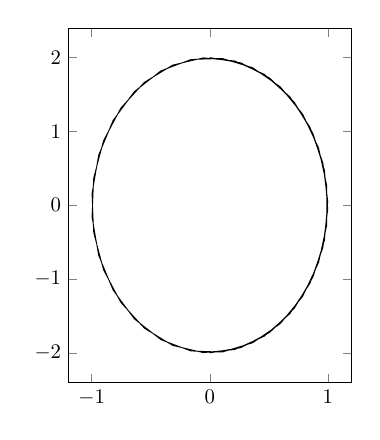
\begin{tikzpicture}[scale = 0.75]
                    \begin{axis}
                    [
                        y=1.25cm,
                        x=2cm,
                        view={60}{30},
                    ]
                    \addplot[
                        domain=0:5*pi,
                        samples = 60,
                        samples y=0,
                    ]
                    ({sin(deg(x))}, {2*cos(deg(x))});
                    \end{axis}
                \end{tikzpicture}
            \end{center}
        \end{wrapfigure}
        \begin{align}
            f(x,y) =& x^2 + \frac{y^2}{4}\\
            \{f(x,y) =& 1\}\text{\;(Level set)}\\
            =& \{(x,y)|x^2 + \frac{y^2}{4} = 1\}
        \end{align}
        Theorem: Given $f(x,y)$ differentiable, then the gradient $\nabla f\perp$ the level set.
        
        We can prove it by using the chain rule: let $\gamma(t)$ be a parametric function of my level set $\{f(x,y) = 1\}$, $f(\gamma(t))=1$ and differentiate both sides.
        \begin{align}
            0 = D(f(\gamma(t))) =& Df(\gamma(t)) D(\gamma(t))\\
            =& \nabla F(\gamma(t))_{1\times2} \cdot (\gamma_1'(t),\gamma_2'(t))_{2\times1}\\
            \text{Hence\;}\Rightarrow& \nabla F(\gamma(t))_{1\times2} \perp (\gamma_1'(t),\gamma_2'(t))_{2\times1}
        \end{align}
        Example: Look at a surface $\sin(xy)-2\cos(yz)=0$ Find the tangent plane of this surface at $(\frac{\pi}{2},1,\frac{\pi}{3})$. The idea is that consider the surface as a level set of $F(x,y,z) = \sin(xy)-2\cos(yz),\{F=0\}$
        
        Using the Theorem: $\nabla F$ is hence perpendicular to this surface, giving us the normal direction of our tangent plane.
        
        \begin{align}
            \nabla F = (\frac{df}{dx},\frac{df}{dy},\frac{df}{dz})
            =& (y\cos(xy),x\cos(xy)+2z\sin(yz),2y\sin(tz))\\
            =& (\cos(\frac{\pi}{2}),\frac{\pi}{2}\cos(\frac{\pi}{2})+\frac{2\pi}{3}\sin(\frac{\pi}{3}),2\sin(\frac{\pi}{3}))\\
            =& (0,\frac{\sqrt{3}\pi}{3},\sqrt{3})\\
            0=&0\cdot(x-\frac{\pi}{2}) + \frac{\sqrt{3}\pi}{3}(y-1)+\sqrt{3}(z-\frac{\pi}{3})
        \end{align}
        Where the last equation above is the equation of the tangent plane.
        
    \subsection{Parametric Curves}
        \dots are vector functions in 1 variable.
        
        Definition: A parametric curve in $\R^n$ is a vector valued function where $\vec{c}(t):R^1\rightarrow\R^n$
        
        All the component functions of $\vec{c}(t)$ are functions in 1 variable.
        
        Example:
        
        1) Draws a Circle
        \begin{align}
            \vec{c}(t) = (\cos(t),\sin(t)),t\in[0,2\pi]
        \end{align}
        2) Draws a eclipse at plane z = 3
        \begin{align}
            \vec{c}(t) = (a\cos(t),b\sin(t),3),t\in[0,2\pi]
        \end{align}
        3) Eclipse spiraling up
        \begin{align}
            \vec{c}(t) = (a\cos(t),b\sin(t),t),t\in[0,2\pi]
        \end{align}
        
        Definition: Orientation of $\vec{c}(t)$, the direction corresponding to increasing t-value is called the positive orientation of $\vec{c}(t)$. The opposite direction is the negative orientation.
        
        Example: Positive orientation = Clockwise
        \begin{align}
            \vec{c}(t) = (\cos(t),-\sin(t),t),t\in[0,2\pi]
        \end{align}
        
        Derivative of $\vec{c}(t)$
        
        If $\vec{c}(t) = (x(t),y(t),z(t))$, $\vec{c'}(t) = (x'(t),y'(t),z'(t))$
        
        \begin{enumerate}
            \item $\vec{c}(t)$ is a vector function
            \item $\vec{c'}(t)$ is a tangent to curve $\vec{c}(t)$
        \end{enumerate}
        
        Terminology: $\vec{c'}(t)$ is the velocity of $\vec{c}(t)$, and $|\vec{c'}(t)|$ is the speed of $\vec{c}(t)$. The speed of the curve $\vec{c}(t) = (\cos(t), \sin(t))$ for example, is 1.\\
        
        What is the length of curve $\vec{c}(t) = (\cos(t),\sin(t),t)$ between (0 to 2$\pi$)Given $\vec{c}(t)$ differentiable between range a and b, length of the curve would be
        
        \begin{align}
            l =& \int^{b}_{a}{|\vec{c'}(t)|}dt\\
            |\vec{c'}(t)| =& \sqrt{\sin(t)^2 + \cos(t)^2 + 1} = \sqrt{2}\\
            l =& \int^{2\pi}_{0}{\sqrt{2}dt}
        \end{align}
        Think of length as a function in t
        \begin{align}
            l(t) = \int^{t}_{a}{|\vec{c'}(x)|}dx
        \end{align}
        If curve $\vec{c}(t)$ differentiable and $\vec{c}(t) \neq 0$,
        \begin{enumerate}
            \item $|\vec{c'}(t)| > 0$
            \item $l(t)$ strictly increasing.
            \item l is one to one function so has inverse.
        \end{enumerate}
        \begin{align}
            l[a,b] \rightarrow& \R^1,\text{\;l has an inverse.}\\
            t\rightarrow& l(t),\text{\;think of our parameter t}\\
        \end{align}
        t can now be expressed as a function in terms of length, $\vec{c}(t) = \vec{c}(t(l)) = \vec{c'}(l)\\$
        
        Proof:
        
        In our last example of calculating length, we can find an inverse for $l(t) = \sqrt{2}t$ resulting $t = \frac{l}{\sqrt{2}}$, by substitution we can reparameterize $\vec{c}(t)$ into $\vec{c}(l)$\\
        
        \begin{align}
            c(l) =& \vec{c}(t(l))\\
            \frac{d\vec{c}(l)}{dl} =& \frac{\vec{c}(t(l))}{dt}\cdot\frac{dt}{dl}\\
            =&\vec{c'}(t)\cdot\frac{1}{|\vec{c'}(t)|}\\
            |\frac{d\vec{c}(l)}{dl}|=&|\vec{c'}(t)|\cdot\frac{1}{|\vec{c'}(t)|}=1
        \end{align}

    \subsection{Acceleration}
        Acceleration is the second derivatives of length, hence the definition of second derivative can be expressed as below:\\
        
        Definition: Given $\vec{c}(t)$, $\vec{a}(t) = \vec{c''}(t)$ the acceleration of $\vec{c}$.\\
        
        Example:
        
        1) Ellipse
        \begin{align}
            \vec{c_1}(t) =& (\cos(t),2\sin(t)), t\in[0,2\pi]\\
            \vec{c_1'}(t) =& (-\sin(t),2\cos(t))\\
            \vec{c_1''}(t) =& (-\cos(t),-2\sin(t))
        \end{align}
        
        2) Different para of the same Ellipse
        \begin{align}
            \vec{c_2}(t) =& (\cos(t^2),2\sin(t^2)), t\in[0,\sqrt{2\pi}]\\
            \vec{c_2'}(t) =& 2t(-\sin(t^2),2\cos(t^2))\\
            \vec{c_2''}(t) =& (-2\cos(t^2)-4t^2cos(t^2),4cos(t^2)-8t^2\sin(t^2))
        \end{align}
        
        Facts:
        \begin{enumerate}
            \item We can have different parameterations of a curve
            \item Velocity, acceleration depend on the para we choose in general
            \item For different parameterization $\vec{c_1}$, $\vec{c_2}$ of the same curve, $\vec{c_1'}(t)\parallelsum\vec{c_2'}(t)$
            \item "Unit Velocity" $\frac{\vec{c_1'}(t)}{|\vec{c_1'}(t)|}=\pm\frac{\vec{c_2'}(t)}{|\vec{c_2'}(t)|}$ are equal, the $\pm$ depends on the orientations of the $\vec{c_1}$ and $\vec{c_2}$.
        \end{enumerate}
        
        Definition:Given $\vec{c}(t)$, assume $|\vec{c'}(t)|\neq0$, defined the unit tangent vector $\vec{T}(t) = \frac{\vec{c'}(t)}{|\vec{c'}(t)|}$. If $\vec{c_1}(t)$ and $\vec{c_2}(t)$ are two different parameter of a curve with the same orientation, their unit tangent vector equals.
    \subsection{Curvature}
        Idea: Curvature is a measure of how sharply a curve is bending at a point, it is the "rate of change" of directions along a curve. So a straight line has no curvature, and a slightly curved line has a small curvature.\\
        
        Definition: Quantitatively, if $\vec{c}(t)$ is parametered by length, (namely, $|\vec{c}(t)|=1$), then we define the curvature at $l=l_0$ to be $k(l_0)=|\vec{c''}(l_0)|=|\frac{d^2\vec{c}(l)}{dl^2}|_{l=l_0}$\\
        
        Remark: IF $\vec{c}(t)$ not parametered by length, then $|\vec{c''}(t)|$ is not the curvature.\\
        
        Explanation: a curve is like a highway and a parameterized function $\vec{c}(t)$ is like someone driving along this highway giving his position vector at a given time. Parameterized by length would be driving at a constant/normalized speed. A curvature is how sharp a turn is, measured by looking at how quickly the driver need to turn their steering wheel.\\
        
        Generally, $|\vec{c'}(l)| = 1\Rightarrow\vec{c'}(l)$ unit tangent, so $\vec{c''}(t)$ is curvature.\\
        
        Example:
        
        1)Find parameter by length
        \begin{align}
            \vec{c}(t) =& \vec{a} + t\vec{v}\\
            \text{Constant vectors:\;}& \vec{a} = (1,2,3),\vec{v}=(0,2,1)\nonumber\\
            \text{Length function\;}l(t) =& \int^{t}_{0}|\vec{c'}(x)|dx\\
            =& \int^{t}_{0} |\vec{v}|dx,\;\;\vec{v}=(0,2,1)\\
            l =& l(t) = \sqrt{5} t\\
            t =& t(l) = \frac{l}{\sqrt{5}}
        \end{align}
        Curvature would be zero since it is a line, its second derivative would be a zero.\\
        
        2) Find the curvature for a circle
        \begin{align}
            \vec{c}(t) =& (r\cos(t),r\sin(t)), r>0 \text{\;circle\;} x^2 + y^2 = r^2\\
            \text{length function\;\;}l(t) =& \int^{t}_{0} |\vec{c'}(x)|dx = rt\\
            t(l) =& \frac{l}{t}\\
            \vec{c}(l) =& (r\cos(\frac{l}{r}),r\sin(\frac{l}{r}))\\
            \vec{c''}(l) =& (-\frac{\cos(l/r)}{r},-\frac{\sin(l/r)}{r})\\
            k(l) =& |\vec{c''}(l)|\\
            =& \sqrt{(-\frac{\cos(l/r)}{r})^2+(-\frac{\sin(l/r)}{r})^2} = \frac{1}{r}
        \end{align}
        Curvature for circle of radius $r =\frac{1}{r}$\\
        
        Second Definition of Curvature:
        
        If $\vec{c}(t)$ any parameteric curve, $\vec{c'}(t)\neq0$, recall the unit tangent vector $\vec{T} = \frac{\vec{c'}(t)}{|\vec{c'}(t)|}$, then define curvature $k(t)=\frac{|\vec{T'}(t)|}{|\vec{c'}(t)|}$
        
        Theorem: Definition 1 and 2 of curvature are the same.
        \begin{align}
            \vec{c'}(t) = \frac{d\vec{c}(t(l))}{dt}\\
            =&\frac{d\vec{c}(t)}{dt}\cdot\frac{dt}{dl}\\
            =&\frac{\vec{c'}(t)}{|\vec{c}(t)|} = \vec{T}\\
            k(l(t)) = |\vec{c''}(t)| =& |\frac{d^2\vec{c}}{dl^2}| = |\frac{d\vec{T}(t(l))}{dl}|\\
            =&\frac{d\vec{c}(t)}{dt}\cdot\frac{dt}{dl}\\
            =&|T'(t)|\cdot\frac{1}{|\vec{c'}(t)|} = k(t)
        \end{align}
        
        Using the second definition to find the curvature of the parabola $y = x^2$
        \begin{align}
            \vec{c} =& (t,t^2)\\
            \vec{c'}(t) =& (1,2t)\\
            \vec{T}(t) =& \frac{(1,2t)}{\sqrt{1+4t^2}}\\
            \vec{T'}(t) =& \frac{(0,2)}{\sqrt{1+4t^2}} + (1,2t)\cdot((a+4t^2)^{-\frac{1}{2}})'\\
            =& \frac{(-4t,2)}{(1+4t^2)^\frac{3}{2}}\\
            |T'(t)| =& \frac{\sqrt{4+16t^2}}{(1+4t^2)^{\frac{3}{2}}}\\
            =& \frac{2}{1+4t^2}\\
            K(t) =& |T'(t)|\cdot\frac{1}{|c'(t)|}\\
            =& \frac{2}{(1+4t^2)} \cdot\frac{1}{\sqrt{1+4t^2}}\\
            =& 2\cdot(1+4t^2)^{-\frac{3}{2}}
        \end{align}
        As $x$ approaches $\infty$, the curvature approaches 0, $y=x^2$ became more like a straight line.\\
        
        Osculating Plane and Circle
        \begin{enumerate}
            \item Derivative --- Tangent line
            \item Curvature  --- Osculating Circle
        \end{enumerate}
        
        Observations:
        
        1) If $\vec{c}(l)$ parameterized by length, then
        \begin{align}
            \vec{c'}(l) \perp&\; \vec{c''}(l)\\
            \because (\vec{c'}(l)\cdot\vec{c'}(l))' =& (|\vec{c}(l)|^2)' = (1)'\\
             \vec{c'}(l)\cdot\vec{c''}(l) + \vec{c'}(l)\cdot\vec{c''}(l)=& 0\\
             \Rightarrow \vec{c'}(l)\cdot\vec{c''}(l) =& 0
        \end{align}
        so second derivative is the normal and the first derivative is the tangent.
        
        2) If $\vec{c}$(t) is any parameterized curve, its unit tangent vector T and T' is
        \begin{align}
            \vec{T}(t) =& \frac{\vec{c'}(t)}{|\vec{c'}(t)|}\\\
            \because (\vec{T}(t)\cdot\vec{T}(t))' =& (|\vec{T}(t)|^2)' = (1)'\\
            \Rightarrow \vec{T}(t)\cdot\vec{T'}(t) =& 0\\
            \therefore \vec{T}(l) \perp&\; \vec{T'}(l)
        \end{align}
        
        Definition: Osculating Plane: Given $\vec{c}(t),\;\vec{c}(t)\neq0$, then the osculating plane is the plane spanned by $\vec{T}(t)$ and $\vec{T'}(t)\\$
        
        Recall that we computed for a circle with radius $r$ its curvature $k = \frac{1}{r}$, therefore, if have a $\vec{c}(t)$ with $k(t_0) = k$, then at this point, the curve $\vec{c}(t)$ is "modeled" by a circle of radius $\frac{1}{k}\\$
        
        Definition: Osculating Circle: Given $\vec{c}(t), \vec{c'}(t)\neq0$, then the osculating circle of $\vec{c}$ at $t=t_0$ is a circle on the osculating plane at $t=t_0$ and has radius $\frac{1}{k(t_0)}$, and the tangent to the curve. (The best approximation of the curve at that point by the circle)\\
        
        Example: Find the equation of the osculating plane at $\vec{c}(\pi) = (-a,0,b\pi)$ of $\vec{c}(t) = (a\cos(t), a\sin(t), bt)\;,t\geq0;\;a,b>0$, 
        \begin{align}
            \vec{T}=&\frac{\vec{c'}(t)}{|\vec{c'}(t)|}=\frac{(-a\sin(t), a\cos(t), b)}{\sqrt{a^2 + b^2}}\\
            \vec{T'} =& \frac{(-a\cos(t), -a\sin(t), 0)}{\sqrt{a^2 + b^2}}\\
            \text{Osc.Plane} =& \vec{T}\times\vec{T'}\\
            =& \frac{1}{a^2+b^2} (ab\sin(t), -ab\cos(t),a^2)|_{t=\pi}\\
            =& \frac{1}{a^2+b^2}(0,ab,a^2)\\
            \text{calculating plane at given point}\;\;&\nonumber\\
            a^2b\pi =& 0x + aby + a^2z
        \end{align}
    \subsection{Higher order derivatives and Taylor expansions}
        Recall partial derivatives of $F(x,y)$ by x and y denoted by $F_x$ and $F_y$, second order derivative = $F_{xx}$ and $F_{yy}$, first x then y $F_{xy}$ and first y then x $F_{yx}$, vise versa. \\
        
        Theorem: If $F(x,y)$ differentiable and $F_{xy}$, $F_{yx}$ continuous, $F_{xy}=F_{yx}$, hence the order can be switched\\
        
        Example: $f(x,y,z) = x^2e^{y^2-x}+x^2yz^2-cos(x^2+y^2),\; f_{xzzy} = ?$ switch order, try finding $f_{zzxy}$ instead
        \begin{align}
            df/dz = f_z = 2zx^2y \Rightarrow fzz = {2x^2y} \Rightarrow f_{zzxy} = 4x
        \end{align}
    \subsection{Taylor Expansions}
        One Variable: $y = f(x),\;f'(x) = $, tangent line of graph of the function, its linear approximation at point $x=x_0$, equation of tangent line is $y = f(x_0) + f'(x_0)(x-x_0)$. Higher order $f'(x)\rightarrow$ higher degree approximation. 
        
        \begin{align}
            f(x) - f(x_0) =& \int^{x}_{x_0} f'(t)dt\\
            \int u'v =& uv - \int v'u,\;u=t,v=f'(t)\\
            =&tf'(t)|_{x_0}^{x} - \int^{x}_{x_0}tdf'(t)\text{\;by parts}\\
            =&[xf'(x) - x_0 f'(x_0)] - \int^{x}_{x_0}tf''(t)dt\\
            =&(xf'x - xf'(x_0)) + (xf'x_0 - x_0f'(x_0))- \int^{x}_{x_0}tf''(t)dt\\
            =&(x-x_0)f'(x_0)+x(f'(x)-f'(x_0)) - x\int^{x}_{x_0}tf''(t)dt\\
            =&f'(x_0)(x-x_0) + x\int^{x}_{x_0}f''(t)dt - \int^{x}_{x_0}tf''(t)dt\\
            f(x) =& f(x_0) + f'(x_0)(x-x_0) + \int^{x}_{x_0}(x-t)f''(t)dt\\
        \end{align}
        This is the 1 st Taylor expansion where $f(x_0) + f'(x_0)(x-x_0)$ is the 1st order approximation, a tangent line, and $\int^{x}_{x_0}(x-t)f''(t)dt$ is the 1st order remainder. error/diff. to linear approx.\\
        
        We can continue to get a higher order Taylor expansion using integration by parts by setting $v=f''(t)$ and $u' = (x-t)$ which would yield:
        \begin{align}
            f(x) =& f(x_0)+f'(x_0)(x-x_0)\\\nonumber
            &+ f''(x_0)\cdot\frac{(x-x_0)^2}{2} \\\nonumber
            &+ \int^{x}_{x_0}(x-t)f'''(t)\cdot\frac{(x-t)^2}{2}dt
        \end{align}
        
        Theorem: if $f(x)$ differentiable, then $\frac{d^n(f(x))}{dx^n}$ exists for all n. Hence the n-th order of the Taylor expansion would be:
        \begin{align}
            f(x) =& f(x_0)+\frac{f'(x_0)(x-x_0)}{1!} + \frac{f''(x_0)(x-x_0)}{2!} \dots\\\nonumber
            &+ f^{(n)}(x_0)\frac{(x-x_0)^n}{n!} + \int^{x}_{x_0}(x-t)f^{(n+1)}(t)\cdot\frac{(x-t)^n}{n!}dt
        \end{align}
        Example:
        
        Find the 2nd order Taylor expansion at $x = 0$ of $f(x) = x+e^{-2x}$ USe that to approximate the value $f(0.075) = 0.075 + e^{-0.15}$ and estimate the error.
        \begin{align}
            f'(x) =& (1-2e^{2x}), f''(x) = 4e^{-2x}\\\nonumber
            f(x) =& f(0) + f'(0)(x-0)\\\nonumber
            &+ \frac{f''(0)(x-0)^2}{2}\\\nonumber
            &+ \int^{x}_{0}f'''(t) \frac{(x-t)^2}{2}dt\\\nonumber
            f(0.075)\approx&1-(0.075)+2(0.075)^2
        \end{align}
        Error given y the remainder $R(x)$, a bound for the error
        \begin{align}
            \text{error}\leq|R(x)| \leq& \left|\int^{x}_{0}-8e^{2t}\cdot\frac{(x-t)^2}{2}dt\right|\\
            \leq& 4x^2 (x-0) = 4x^3 = (4\cdot(0.075)^3)
        \end{align}
        For 2 dimension, the second order expansion of $F(x,y)$ at $(x_0,y_0)$ is:
        \begin{align}
            F(x,y) =& F(x_0,y_0) \\\nonumber
            &+ \frac{1}{1!}\left[\frac{\sigma F}{\sigma x}(x_0,y_0)(x-x_0) + \frac{\sigma F}{\sigma y}(x_0,y_0)(y-y_0)\right]\\\nonumber
            &+ \frac{1}{2!}\left[\frac{\sigma^2 F}{\sigma x^2}(x_0,y_0)(x-x_0) + \frac{\sigma^2 F}{\sigma y^2}(x_0,y_0)(y-y_0)\right.\\\nonumber
            &+ \left. 2\frac{\sigma ^2 F}{\sigma x\sigma y}\right] + R_2(x,y)
        \end{align}
        Example: Find the second Taylor expansion of $f(x,y) = sin(x+y) + cos(x-3y)$ at (0,0)
        \begin{align}
            f_x =& \cos(x+y)-\sin(x-3y)\\
            f_y =& \cos(x+y)+3\sin(x-3y)\\
            f_{xx} =& -\sin(x+y) - \cos(x-3y)\\
            f_{xy} =& -\sin(x+y) + 3\cos(x-3y)\\
            f_{yy} =& -\sin(x+y) - 9\cos(x-3y)\\
            f(x,y) =& f(0,0) + f_x(0,0)x + f_y(0,0)y\\
            +& \frac{1}{2}\left[f_{xx}x^2 + f_{yy}y^2 + 2f_{x,y}xy\right] + R_2(x,y)\\
            =& 1 + x + y + \frac{1}{2}(-x^2 - 9y^2 + 6xy) + R_2(x,y)
        \end{align}
        Second Approximation, Taylor Polynomial.\\
        
        For extreme values of F(x,y): Recall that given y = f(x), differentiable, n-th Taylor expansion at $x = x_0$
        \begin{align}
            f(x) =& f(x_0) + f'(x_0)(x-x_0) + f''(x_0)\cdot\frac{(x-x0)^2}{2}\;\dots\\
            &+ f^{(n)}(x_0)\frac{(x-x_0)^n}{n!}\;\text{Taylor polynomial}\\
            &+ \int^{x}_{x_0}f^(n+1)(t)\frac{(x-t)^n}{n!}dt\;R_n(x)\text{remainder}
        \end{align}
        Taylor Expansion for $F(x,y)$ at $(x_0,y_0)$
        \begin{align}
            F(x,y) =& F(x_0,y_0) + F_x(x_0,y_0)x + F_y(x_0,y_0)y\\
            &+ F_{xx}(x_0,y_0)\frac{x^2}{2} + F_{xy}(x_0,y_0)\frac{xy}{2}\\
            &+ F_{yx}(x_0,y_0)\frac{yx}{2} + F_{yy}(x_0,y_0)\frac{y^2}{2}\\
            &+ R_2(x,y)
        \end{align}
        Recall: for $y=f(x)$, critical points, $f'(x_0) = 0$ are candidates for local max and local min.
        \begin{enumerate}
            \item $f''(x_0) > 0$ local min
            \item $f''(x_0) < 0$ local max
            \item $f''(x_0) = 0$ inconclusive
        \end{enumerate}
        if $x_0$ is critical point, first derivative term $f'(x_0) = 0$ removed from polynomial. 
        
        The two variable are F(x,y). Definition F(x,y) differentiable, then say $(x_0,y_0)$ is a critical point if $\nabla F(x_0,y_0) = 0$.
        
        Recall equation of tangent plane
        \begin{align}
            z = F(x_0,y_0) + F_x(x_0,y_0)(x-x_0) + F_y(y-y_0)
        \end{align}
        Tangent plane is horizontal. Definition: for $F(x,y)$, define the Hessian matrix.
        \begin{equation}
            \begin{pmatrix}
                F_{xx} & F_{xy}\\
                F_{yx} & F_{yy}
            \end{pmatrix}(x_0,y_0)
        \end{equation}
        Define the discrimanant, $(x_0,y_0)$ is critical point. 
        \begin{equation}
            D(x_0,y_0) = det
            \begin{pmatrix}
                F_{xx}(x_0,y_0) & F_{xy}(x_0,y_0)\\
                F_{yx}(x_0,y_0) & F_{yy}(x_0,y_0)
            \end{pmatrix}(x_0,y_0)
            = F_{xx}F_{yy} - F_{xy}F_{yx}
        \end{equation}
        Theorem (2nd derivative test): Suppose $(x_0,y_0)$ is a critical point, then
        \begin{enumerate}
            \item If $D(x_0,y_0)>0$ and $F_{xx}>0$ or $(F_{yy} > 0)$, then $(x_0,y_0)$ is a local minimum
            \item If $D(x_0,y_0)>0$ and $F_{xx}<0$ or $(F_{yy} < 0)$, then $(x_0,y_0)$ is a local maximum
            \item if $D(x_0,y_0)<0$, then $(x_0,y_0)$ is a saddle point.
            \item if $D(x_0,y_0)=0$, then it is inconclusive.
        \end{enumerate}
        Find and classify all critical points of $F(x,y) = x^3 -3x^2 -3y^2 + 3xy^2$
        \begin{align}
            F_x =& 3x^2 - 6x + 3y^2 = 0\\
            F_y =& -6y + 6xy = 0\\
            \Rightarrow\;y=&0\;or\;x=1 \text{\;giving two critical point}\\
            y=0,\Rightarrow&(0,0),(2,0)\\
            x=1,\Rightarrow&(1,1),(1,-1)
        \end{align}
        Use Second derivative to test for the four critical points
        \begin{align}
            D(x,y) =& F_{xx}F_{yy} - F_{xy}^2\\
            D(1,1) =& \Rightarrow\text{ is a saddle point}\\
            D(1,-1)=& \Rightarrow\text{ is a saddle point}\\
            D(0,0) =& \Rightarrow\text{ is local max}\\
            D(2,0) =& \Rightarrow\text{ is local min}
        \end{align}
        Why is this true?
        
        From the second Taylor expansion, at a critical point, the dominant part:
        \begin{align}
            F_{xx}(x_0,y_0)(x-x_0)^2 + 2F_{xy}(x_0,y_0)(x-x_0)(y-y_0)+F_{yy}(y-y_0)^2
        \end{align}
        Homogeneous degree 2 polynomial in 2 variables:
        \begin{align}
            P(x,y) =& ax^2 + 2Cxy + by^2\\
            =&a(x^2 + \frac{2c}{a}xy + \frac{b}{a}y^2)\\
            =&a((x-\frac{c}{a}y)^2 + \frac{ab-c^2}{a^2}y^2)\\
            =&a((x-\frac{c}{a}y)^2 + \frac{ab-c^2}{a^2}y^2)\\
            \Delta =& ab-c^2 > 0, \text{then}\begin{cases}
                x'=x-\frac{c}{a}y\\
                y'=x-\frac{\sqrt{ab-c^2}}{a}y
            \end{cases}\\
            =& a((x')^2 + (y')^2)\\
            &\Rightarrow a > 0 \text{ local min, }a < 0 \text{ local max}\\
            \text{If }\Delta <& 0 \begin{cases}
                x'=x-\frac{c}{a}y\\
                y'=x-\frac{\sqrt{c^2-ab}}{a}y
            \end{cases}
        \end{align}
        \begin{align}
            \text{then } P(x,y) =& P(x', y') = a((x')^2-(y')^2)\\
            a>&0 \text{ saddle point}
        \end{align}
        Apply this to $F_{xx}(x_0,y_0)(x-x_0)^2 + 2F_{xy}(x_0,y_0)(x-x_0)(y-y_0)+F_{yy}(y-y_0)^2$
        \begin{align}
             a =& F_{xx}(x_0,y_0)(x-x_0)^2\\
             b =& F_{yy}(x_0,y_0)(x-x_0)^2\\ 
            2c =& 2F_{xy}(x_0,y_0)(x-x_0)^2\\
            ab-c^2 =& D(x,y)
        \end{align}
        Global Extreme Values for F(x,y).
        
        Recall local max/min:
        \begin{enumerate}
            \item Find critical points $\nabla F(x_0,y_0)=\vec{0}$
            \item Use second derivatives to test the critical points.
        \end{enumerate}
        For Global Extreme values:\\
        
        Example: \\
        
        1) Find global min and max of $f(x,y) = x^3-3xy + 3y^2$ defined on the rectangle $D = \{(x,y)|0\leq x\leq 1, 0\leq y \leq2\\$ First, find local critical point
        \begin{align}
            f_x =& 3x^2 - 3y = 0\\
            f_y =& -3x + 6y = 0\\
            &\Rightarrow x = 2y\\
            \text{plug in to }f_x:\;0 =& 3(4y^2-y)\\
            0 =& y(4y-1)\\
            &\Rightarrow y=0 \text{ or } y=\frac{1}{4}\\
            \therefore (0,0)\;\&\;(0.5,0.25)& \text{ two critical point}\\
            \text{Hessian Matrix }D(x,y) =& det\left[\begin{array}{cc}
                                                fxx & fxy\\
                                                fxy & fyy
                                            \end{array}\right]\\
            =& f_{xx} - f_{xy}^2 = 36x-9 = 9(4x - 1)\\
            &\Rightarrow D(0,0) = -9 < 0,\text{ saddle, neither max/min}\\
            &\Rightarrow D(0.5,0.25) = 9 > 0,\;f_{xx}(0.5,0.25) = 3>0\\
        \end{align}
        Need to compare with boundary values.
        \begin{align}
            \text{Side 1: }\{x=0,\;& 0\leq y\leq2\}\\
            f(x,y) =& x^3 - 3xy + 3y^2|{x=0}\\
            f(0,y) =& 3y^2 \Rightarrow\text{ max 12 min 0}\\
            \text{Side 2: }\{y=0,\;& 0\leq x\leq1\}\\
            f(x,0) =& x^3,\text{ max 1 min 0}\\ 
            \text{Side 3: }\{x=1,\;& 0\leq y\leq2\}\\
            f(1,y) =& 1-3y+3y^2,\text{ max 7 min 0.25}\\
            \text{Side 4: }\{y=2,\;& 0\leq x\leq1\}\\
            f(x,2) =& x^3-6x+12,\text{ max 12 min 7}
        \end{align}
        Hence global max 12 at (0,2) and -1/16 at (0.5,0.25)
        
        2)Find for the function $f(x,y) = 2x^2 + 2y^2 - x + y$ on disk $D = \{(x,y): x^2 + y^2 \leq 1\}$ its global Max and min/min
        \begin{align}
            f_x =& 4x - 1, f_y = 4y + 1,\\
            f_x =& 0\text{ and }f_y = 0\rightarrow (x=1/4,y=-1/4)\\
            f_{xx} =& 4, f_{yy} = 4, f_{xy} = 0\\
            D(x,y) =& 16-0^2 = 16 > 0, f_{xx} = 4 > 0\\
            \text{see } (x= 1/4, y=-1/4)&\text{ is local min}\\
            \text{Parameterize the } & \text{ bounding (unit circle)}\nonumber\\
            \vec{c}(t) =& (\cos(t),\sin(t)), t\in[0,2\pi]\\
            \text{plugin } f(\cos(t),\sin(t)) =& 2-\cos(t)+\sin(t),\;t\in[0,2\pi]\\
            f'(t) =& \sin(t) + \cos(t) = 0\\
            -1 =& \tan(t)\\
            \therefore \text{critical points} t =& \frac{3\pi}{4}, t = \frac{7\pi}{4}\\
            f(t) =& 2-cos(t) + sin(t)\text{ at } 0 \& 2\pi = 1 \& 1\\
            f(\frac{3\pi}{4}) =& 2-\cos(\frac{3\pi}{4})+\sin(\frac{3\pi}{4})=2+\sqrt{2}\\
            f(\frac{7\pi}{4}) =& 2-\sqrt{2}\text{ min on boundary}
        \end{align}
        
        Recall have local min at (0.25,-0.25)\\
        Global max at $(-\frac{\sqrt{2}}{2},\frac{\sqrt{2}}{2}),\;2+ \sqrt{2}$\\
        Global max at $(\frac{1}{4},-\frac{1}{4}),\;-\frac{1}{4}$\\
        Optimization with constraint --- Lagrangian multiplier.\\
        
        Given f(x,y), find max/min with a constraint g(x,y) = k, k = a fixed number. The langrangian multiplier method would be:
        
        \begin{align}
            \text{Step 1} \begin{cases}
                \nabla f = \lambda \nabla g, \lambda\text{ = constant}\\
                g(x,y) = k
            \end{cases}
        \end{align}
        solve this system of equation to get (x,y)\\
        Step 2, plug in (x,y) into f(x,y)\\
        
        Example: $f(x,y) = 4xy$, find max/min with condition $x^2 + y^2 = 4$
        \begin{align}
            g(x,y) =& x^2 + y^2, g(x,y) = 4\\
            f\&g=&\begin{cases}
                \nabla f =& (2y,2x) = \lambda\cdot\nabla g = (2x,2y)\\
                g(x,y) =& 4 = x^2 + y^2
            \end{cases}\\
            \therefore 2y =& \lambda 2x \rightarrow \lambda = \frac{y}{x}\\
             2x =& \lambda 2y \rightarrow \lambda = \frac{x}{y}\\
            \therefore x^2 =& y^2 \& g(x,y):x^2+y^2 = 4, x^2 = y^2 = 2\\
            x, y =& \pm \sqrt{2}\text{, 4 solutions, max 8, min -8}
        \end{align}
        Why does it work? at max $\nabla g \parallelsum \nabla f$
    \subsection{Vector Field and Flow}
        Definition: A vector field $\vec{F}:\R^m \rightarrow \R^m$
        \begin{enumerate}
            \item Example 1: $\vec{F}(x,y) = (x,y), \R^2\rightarrow \R^2$
            \item Example 2: $\vec{F}(x,y) = (-y,x) \R^2\rightarrow \R^2$
            \item Example 3: $\vec{F}(x,y,z)=(x^3,xy,e^{xyz})\R^3\rightarrow \R^3$
        \end{enumerate}
        Definition: (Flow/Integral Curve) Given $\vec{F}:\R^m \rightarrow \R^m$, a flow of $\vec{F}$ is  curve $\vec{C}(t):\R^1\rightarrow\R^m$ such that $\vec{C'}(t) = \vec{F}(\vec{C}(t))\\$
        
        Example:
        \begin{align}
            \vec{F}(x,y) = (-y,x)
        \end{align}
        Verify that the curve $\vec{C}(t) = (cos(t),sin(t))$, is a flow/integral curve of $\vec{F}$ by checking if $\vec{C'}(t) = \vec{F}(\vec{C}(t))$
        \begin{align}
            \vec{C'}(t) &= (-sin(t),cos(t))\\
            \vec{C'}(t) &\equiv \vec{F}(\vec{C}(t))
        \end{align}
        
        Remark: Finding flows of a vector field is the focus of differential equations.
        
        An important class of example of vector field is given by $\nabla F$ where $F:\R^m\rightarrow\R^1$, $\nabla F=(\frac{\sigma F}{\sigma x},\frac{\sigma F}{\sigma y},\frac{\sigma F}{\sigma z}):\R^3\rightarrow\R^3$
        
        Looking at $\nabla F$ tells us something about F
        \begin{enumerate}
            \item $\nabla F$ is the direction along which F changes most dramatically.
            \item $\nabla F \perp$ level sets ($F(x,y,z) = c$).
        \end{enumerate}
        Definition (Divergence and Curl): Given $\vec{F}\R^3\rightarrow \R^3$, $\vec{F} = (F_1(x,y,z),F_2(x,y,z),F_3(x,y,z))$. 
        
        Define the divergence of $\vec{F}$
        \begin{enumerate}
            \item div $\vec{F} = (\frac{\sigma F}{\sigma x},\frac{\sigma F}{\sigma y},\frac{\sigma F}{\sigma z})$
            \item div $\vec{F} = \R^3\rightarrow \R^1$ a scalar function
        \end{enumerate}
        Define the curl of $\vec{F}$
        \begin{enumerate}
            \item Curl $\vec{F} = \left[\begin{array}{c}
                \sigma/\sigma x  \\
                \sigma/\sigma y  \\
                \sigma/\sigma z  
            \end{array}\right] \times \left[\begin{array}{c}
                F_1  \\
                F_2  \\
                F_3  
            \end{array}\right]$
            \item div $\vec{F} = \R^3\rightarrow \R^3$ a vector function
        \end{enumerate}
        Easier way to memorize these 2 notations:$\nabla$ is a vector of differential operators $<\frac{\sigma }{\sigma x},\frac{\sigma }{\sigma y},\frac{\sigma }{\sigma z}>$
        
        Hence $\nabla F$ means the gradient of F. So $div\vec{F}$ is the dot product between $\nabla$ and $\vec{F}$: $div\vec{F} = \nabla \cdot \vec{F}$
        
        Hence $\nabla F$ means the gradient of F. So $curl\vec{F}$ is the cross product between $\nabla$ and $\vec{F}$: $curl\vec{F}=\nabla \times \vec{F}$
    
        Similar for two dimension curves, except for the curl, we add a zero to the third dimension making the original function a function plot on a plane in the three dimensional plot. $Curl\vec{F} = curl(F_1,F_2,0)$, and the result will be $(0,0,\frac{\sigma F_2}{\sigma x}-\frac{\sigma F_1}{\sigma y})$, and the scalar curl for $\vec{F}:\R^2\rightarrow\R^2$ is defined as $\frac{\sigma F_2}{x}-\frac{\sigma F_1}{y}$, a scalar function.\\
        
        Meanings of divergence and curl:
        
        Divergence of $\vec{F}$ at $(x_0,y_0)$ is measuring the change of density at this point. Change of volume of flows 
        \begin{align}
            =& F_1(x+\Delta x,y)\Delta y - F_1(x, y)\Delta x\\
            &+\frac{F_2(x,y+\Delta y)\delta x-F_2(x,y)\Delta x}{\Delta x\Delta y}\\
            \approx &\frac{\sigma F_1}{\sigma x}+\frac{\sigma F_2}{\sigma y}div\vec{F}
        \end{align}
        Curl of $\vec{F}:\R^2\rightarrow\R^2$, scalar curl = $\frac{\sigma F_2}{x}-\frac{\sigma F_1}{y}$. is the measurement of the tendency of spin at a point. The Jacobian matrix $D\vec{F}$ capture the instant change of $\vec{F}$ In particular, $D\vec{F}$ capture the infinitely minimal tendency of spin at the point.
        
        A bit about Linear Algebra
        
        If The Jacobian matrix $D\vec{F}$ is symmetric, i.e.$D\vec{F} = D\vec{F}^T$, i.e. $\frac{\sigma F_2}{sigma x} = \frac{\sigma F_1}{sigma y}$. Then $D\vec{F}$ introduces no rotation. Curl measures how far away $D\vec{F}$ from being symmetric, the more asymmetric, the more $D\vec{F}$ rotates a basis. 
        
        Curl in third dimension:
        \begin{enumerate}
            \item $Curl\vec{F}$ = the axis of rotation of $D\vec{F}$. 
            \item $|Curl\vec{F}|$  = rate of rotation of $D\vec{F}$ the instant rate of rotation of $\vec{F}$ at the point.
        \end{enumerate}
        
        Relationship between $\nabla,\;div,\;curl\\$
        \begin{align}
            \R^1 -(\nabla)\rightarrow \R^3 -(curl)\rightarrow \R^3 -(div)\rightarrow \R^1
        \end{align}
        $\R^1 -(\nabla)\rightarrow \R^3$ are both tangent of functions.
        \begin{align}
            curl(\nabla f) =& \vec{0}\\
            div(curl \vec{F}) =& 0
        \end{align}
        
    \subsection{Integration along a path}
    
        Definition: A path (parametric curve) $\vec{c}:[a,b]\rightarrow \R^m$ is $C'$ if $\vec{C}(t)$ exists and is continuous
        
        Definition: A path $\vec{c}:[a,b]\rightarrow \R^m$ is piece-wise $C'$ if can divide $[a,b]$ into finitely many sub-integrals. $[a_1 = a_1, a_2]$, $[a_2, a_3]\dots$, $[a_{n-1}, a_n = b]$ such that $\vec{C} on [a_i,a_{i+1}]$ is $C'$.
        
        Convention:From now on, we assume a path $\vec{C}(t)$ is always piece-wise $C'$.
        
        Definition: If $\vec{C}(t)$ is a piece-wise $C'$ path, we said that
        \begin{enumerate}
            \item $\vec{C}(t)$ is simple if it does not intersect itself or equivalently, $\vec{c}:[a,b]\rightarrow \R^m$ is an 1 to 1.
            \item $\vec{C}(t)$ is simple closed path/curve if there exists $\vec{C}(a) = \vec{C}(b)$ and does not intersect itself except for the 2 end points. 
        \end{enumerate}
        
        Definition: for $\vec{C}:[a,b]\rightarrow \R^m$, $f(x_1\dots x_m): \R^m \rightarrow \R^1$ then integral of f along $\vec{C}$ is denoted by:
        \begin{align}
            \int_{C}f ds=\int_{a}^{b}f\vec{C}(t)\cdot|\vec{C'}(t)|dt
        \end{align}
        Example: Finding the integral of $f(x,y,z) = xyz$ along the path $\vec{C}(t)=(-\sin(t),\sqrt{2}\cos(t),sin(t)), t\in[0,\pi/2]$
        \begin{align}
            \int_c fds =& \int_{0}^{\pi/2}f(\vec{C}(t))\cdot|\vec{C'}(t)|dt\\
            =&\dots\\
            =&-2\int_{0}^{\pi/2} \sin^2(t)\cos(t)dt\\
            =&-\frac{2}{3}
        \end{align}
        Theorem: Path integral of a function does not depend on the parametrization of the path.
        
        Namely, $\vec{C_1}(t)$ and $\vec{C_2}(t)$ are 2 different parameter of the same path, $\int_{C_1} fds = \int_{C_2} fds\\$
        
        The integration of vector field along a path is similar:
        
        Definition: For a path $\vec{c}:[a,b]\rightarrow \R^m$ and a vector function $\vec{F}:\R^m\rightarrow\R^m$ the integral of $\vec{F}$ along $\vec{C}$ is
        \begin{align}
            \int_{\vec{C}}\vec{F}d\vec{s} = \int_a^b \vec{F}(\vec{C}(t))\cdot\vec{C'}(t)dt
        \end{align}
        This can be used in occasion like calculating the work done by a force field.
        
        Example:$\vec{F}(x,y,z) = (-y,x,1)$ force field, and there is a particle moving along a three dimension path $\vec{C}(t)$ and similarly, when the path is perpendicular, work done(hence the integral) would also be zero.\\
        
        1) for $\vec{C}(t) = (t,t,t),\;t\in[0,1]$
        \begin{align}
            \int_{\vec{C}}\vec{F}d\vec{s} =& \int_0^1(-t,t,1)\cdot(1,1,1)dt\\
            =&1\;(J)
        \end{align}
        2) for $\vec{C}(t) = (\cos(t),\sin(t),t),\;t\in[0,2\pi]$
        \begin{align}
            \int_{\vec{C}}\vec{F}d\vec{s} =& \int_0^2\pi(-\sin(t),\cos(t),1)\cdot(-\sin(t),\cos(t),1)dt\\
            =&4\pi\;(J)
        \end{align}
        Properties of $\int_{\vec{C}}\vec{F}d\vec{s}$
        \begin{align}
            \int_{\vec{C}}\vec{F}d\vec{s} =& \int_a^b \vec{F}(\vec{C}(t))\cdot\vec{C'}(t)dt\\
            =& \int_a^b |\vec{F}(\vec{C}(t))|\cdot|\vec{C'}(t)|\cos(\theta t)dt
        \end{align}
        The angle $\theta(t)$ is the angle formed by $\vec{F}(C(t))$, and $\vec{C'}(t)$ is always$< 90$ degree.
        
        If $\vec{F}(c(t)) \perp C'(t)$
        \begin{align}
             \int_{\vec{C}}\vec{F}d\vec{s} = 0
        \end{align}
        If $\vec{C_1}(t)$ and $\vec{C_2}(t)$ are different parametrization of the same path with the same orientation, then
        \begin{align}
            \int_{\vec{C_1}}\vec{F}d\vec{s} = \int_{\vec{C_2}}\vec{F}d\vec{s}
        \end{align}
        If opposite orientation
        \begin{align}
            \int_{\vec{C_1}}\vec{F}d\vec{s} = -\int_{\vec{C_2}}\vec{F}d\vec{s}
        \end{align}
        
        Definition of Circulation: $\vec{C}:[a,b]\rightarrow\R^m$ a simple closed path, for a vector field F, the integration of this vector field along this simple closed path is called the circulation of $\vec{F}$ along C.
        
        For example, along a magnetic field, and such that C is a closed curve, the Ampere's law states that: $\int_c\vec{B}d\vec{s} = \mu I$ where $I$ is the current.
        
        Example: Take for example, the integration of the vector field $\vec{F_1(x,y)}=(-y,x)$ a simple closed path $\vec{C}(t) = (\cos(t),\sin(t)),\;t\in[0,2\pi]$, the circulation would be
        \begin{align}
            \vec{F_1} =& \int_{\vec{C}}\vec{F_1}d\vec{s}\\
            =&\int_{0}^{2\pi}\VectorTwo{-\sin(t)}{cos(t)}\cdot\VectorTwo{-sin(t)}{cos(t)}dt
            =&2\pi
        \end{align}
    
    \subsection{Gradient Vector Field}
        Recall the two different kinds of integrals along a path:
        \begin{align*}
            \int_{\vec{C}}\vec{F}d\vec{s} =& \int_a^b \vec{F}(\vec{C}(t))\cdot\vec{C'}(t)dt, & \int_{C}fds =& \int_a^b \vec{f}(\vec{C}(t))|\vec{C'}(t)|dt
        \end{align*}
        Definition: $\vec{F}:\R^m\rightarrow\R^m$ is called a gradient (conservative) vector field if there exists a function $f:\R^m\rightarrow\R$ such that $\vec{F} = \nabla f$ There are vector fields that are not gradient, recall that $Curl(\nabla f) = 0$:
        \begin{align}
            Curl(\nabla f) =& Curl(\frac{\sigma f}{\sigma x},\frac{\sigma f}{\sigma y})\\
            =&\frac{\sigma{(\sigma f/\sigma y)}}{\sigma x}-\frac{\sigma{(\sigma f/\sigma x)}}{\sigma y}\\
            =&0
        \end{align}
        Hence the curl test: if $\vec{F}:\R^m\rightarrow\R^m,\;curl\vec{F}\neq0$, then $\vec{F}$ cannot be a gradient curve.
        
        Theorem:: Suppose $\vec{F} = \nabla f,\;\vec{C}:[a,b]\rightarrow\R^m$ a path, then
        \begin{align}
            \int_{\vec{C}}\vec{F}d\vec{s} = \int_{\vec{C}}\nabla f d\vec{s} = f(\vec{C}(b))-f(\vec{C}(a))
        \end{align}
        Example: find the integration of a vector field $F = (2x,2e^z,2ye^z)$ along a curve $abc$ $\vec{C}(a) = [0,0,0],\;\vec{C}(b) = [0,-1,1],\;\vec{C}(c) = [1,-1,0]$
        \begin{align}
            \text{Observed that: } \vec{F} = \nabla (x^2+2ye^z) = \nabla f
        \end{align}
        Hence from theorem:
        \begin{align}
            \int_{\vec{C}}\vec{F}d\vec{s} = f(1,-1,0)-f(0,0,0) = -1
        \end{align}
        
        Observations, for two different closed path with the same end points:
        \begin{align}
            \int_{\vec{C_1}}\nabla fds = \int_{\vec{C_2}}\nabla fds
        \end{align}
        equivalently, for a simple closed curve:
        \begin{align}
            \int_{\vec{C}}\vec{F}d\vec{s} = \int_{\vec{C}}\nabla f d\vec{s} = f(\vec{C}(b))-f(\vec{C}(a)) = 0
        \end{align}
        
        Theorem: Hence given a vector field $\vec{F}$, the following statements about it are equivalent:
        \begin{enumerate}
            \item $\vec{F} = \nabla f$
            \item $\int_{\vec{C_1}}\nabla fds = 0$
            \item For any two paths $c_1\;c_2$ with the same end points, $\int_{\vec{C_1}}\vec{F}ds = \int_{\vec{C_2}}\vec{F}ds$
        \end{enumerate}
        
        The curl of $\nabla f = 0$ is a necessary condition for gradient vector field, but is this true such that when $curl \vec{F} = 0$, $\vec{F} = \nabla f$? no
        
        Example: $\vec{F} = (\frac{-y}{x^2+y^2},\frac{x}{x^2+y^2},z)$ (its Curl = 0) defined on $u = \R^3$ (is not simple connected), but if we take a simple closed curve $\vec{c}(t) = (cos(t),sin(t),0)\;t\in[0,2\pi]$, and $\int_{\vec{C}}\vec{F}d\vec{s} \neq 0$, hence not a gradient vector field by theorem.
        
        Definition: Simply connected domains, n belongs to $\R^n$ is said to be simply connected if any closed path can be deformed continuously to a point, u is simple connected. For example, a disk is simply connected and a ring is not as it cannot be shrinked to a simple point.
        
        Theorem: if $\vec{F}:\R^m\rightarrow\R^m$ vector field defined on a simple connected domain and $curl\vec{F} = 0$, then $\vec{F}$ is a gradient vector field.
        
        Proof: supposed that $\vec{u}$ = Disk and $\vec{F}$ defined on u, curl $\vec{F} = 0$, then we claim there exists a function f(x,y) defined on u such that $\nabla f = \vec{F}$
        
        \begin{align}
            \vec{F} =& (F_1(x,y),F_2(x,y)), (a,b) \in u\\
            f(a,b) =& \int_{\vec{C_{a,b}}}\vec{F}d\vec{s}\text{, where }C_{a,b}\text{ is a line }(0,0)---(a,b)\\
            =&\int_0^1(F_1(ta,tb),F_2(ta,tb))\cdot(a,b)dt\begin{cases}C_{a,b}(t) = (ta,tb) t\in[0,1]\end{cases}\\
            =&f(a,b)\\
        \end{align}
        Claim: $\nabla F = \vec{F}$, check for $\frac{\sigma f}{\sigma a}F_1:$
        \begin{align}
            \frac{\sigma f(a,b)}{\sigma a} =& \frac{\sigma }{\sigma a}\int_0^1(F_1(ta,tb),F_2(ta,tb))\cdot(a,b)dt\\
            =& \int_0^1(F_1(ta,tb) + a\frac{\sigma F_1}{\sigma x}\cdot\frac{\sigma x}{\sigma a}+ b\frac{\sigma F_2}{\sigma x}\cdot\frac{\sigma x}{\sigma a} dt,\;x=ta,\;\frac{\sigma x}{\sigma a}=t\\
            Curl \vec{F} =& \frac{\sigma F_2}{\sigma x} - \frac{\sigma F_1}{\sigma y} = 0\\
            =& \int_0^1(F_1(ta,tb) + at\frac{\sigma F_1}{\sigma x}+ bt\frac{\sigma F_1}{\sigma x}dt\\
            &x=at, \frac{\sigma x}{\sigma t} = a, y = bt, \frac{\sigma y}{\sigma t} = b\\
            =&\int_0^1(F_1(ta,tb) + t\frac{\sigma F_1}{\sigma x}\cdot\frac{\sigma x}{\sigma t}+ t\frac{\sigma F_1}{\sigma y}\cdot\frac{\sigma y}{\sigma t} dt\\
            =&\int_0^1(F_1(a,b)+t \frac{df}{dt})dt\\
            =&\int_0^1\frac{d}{dt}(t F_1(ta,tb))dt\\
            =&(t F_1(ta,tb))\\
            \frac{\sigma f}{\sigma a} = F_1(a,b)\\
        \end{align}
        Rest can be proved similarly.
        
        Next for arbitrary domain u, assume that $curl\vec{F} = 0$ and we want to show that the integral for any two path with the same end points $\int_{\vec{C_1}}\vec{F}d\vec{s} = \int_{\vec{C_2}}\vec{F}d\vec{s}$
        
        Idea: deform $C_1$ to $C_2$ such that any 2 adjacent curves can be covered by a series of small disks. Because for each disk, we shown $\int F$ independent of paths.
        
        Then
        \begin{align}
            \int_{c_1}\vec{F}ds = \sum_i \int_{P_i}\vec{F}ds = \sum_i \int_{Q_i}\vec{F}ds =  \int_{C_3}\vec{F}ds
        \end{align}
        Similarly: 
        \begin{align}
            \int_{c_1}\vec{F}ds = \int_{C_3}\vec{F}ds = \int_{C_n}\vec{F}ds =  \int_{C_2}\vec{F}ds
        \end{align}
        so $\int\vec{F}$ is indenependent of choice of paths, by theorem 1, $\vec{F}$ is a gradient vector field.
        
\end{document}